\documentclass[14pt, a4paper]{report}
\usepackage{mathtext}
\usepackage[T2A]{fontenc}
\usepackage[utf8]{inputenc}
\usepackage[russian]{babel}
\usepackage{multirow}
\usepackage{slashbox}
\usepackage{makecell}
\usepackage{graphicx}
\usepackage{physics}
\usepackage{amstext}
\usepackage{caption}
\usepackage{subcaption}
\usepackage{cmap}
\usepackage{float}
\usepackage{indentfirst}

\usepackage[a4paper,
            		left=1in,
            		right=1in,
           		 top=1in,
            		bottom=1in,
            		footskip=.25in]{geometry}

\renewcommand{\thesection}{\arabic{section}.}
\renewcommand{\thesubsection}{\arabic{section}.\arabic{subsection}.}

\title{\textbf{Отчет о выполнении лабораторной работы 2.1 "Опыт Франка-Герца"}}
\author{Калашников Михаил, Б03-202}
\date{}

\begin{document}
\maketitle

\textbf{Цель работы:}
Измерение энергиии первого уровня атома гелия методом электронного возбуждения в динамическом и статическом режимах.
\newline

\section{Теоретические сведения}

Опыт Франка и Герца является одним из самых простых опытов, подтверждающих существование дискретных уровней энергии атомов.

Разреженный гелий заполняет трехэлектродную лампу. Электроны ускоряются в постоянном электрическом поле, созданным между катодом и анодом лампы. Передвигаясь от катода к аноду, электроны сталкиваются с атомами гелия. При энергии, недостаточной для ионизации атома гелия, происходят упругии соударения, при которых электроны практически не теряют энергии.

\begin{figure}[H]
\centering
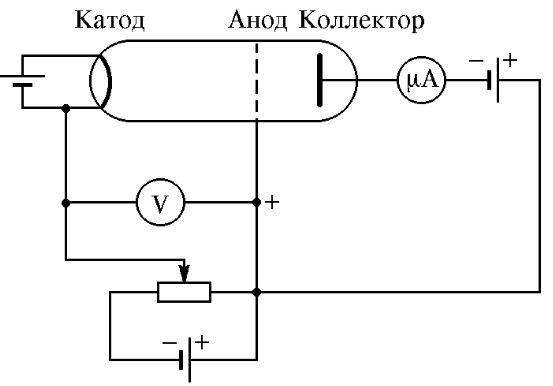
\includegraphics[scale=0.6]{../images/521-1}
\caption{Принципиальная схема опыта Франка и Герца}
\end{figure}

По мере увеличения разности потенциалов между анодом и катодом энергия электронов становится достаточной для возбуждения атомов. При таких неупругих столкновениях кинетическая энергия налетающего электрона передается одному из атомных электронов, вызывая его переход на свободный энергетический уровень или совсем отрывая его от атома.

При увеличении потенциала анода ток коллектора вначале растет. Однако, когда энергия электронов становится достаточной для возбужения атомов, ток коллектора резко уменьшается из-за того, что претерпевшие неупругое соударение электроны не могут преодолеть задерживающее напряжение.

\begin{figure}[H]
\centering
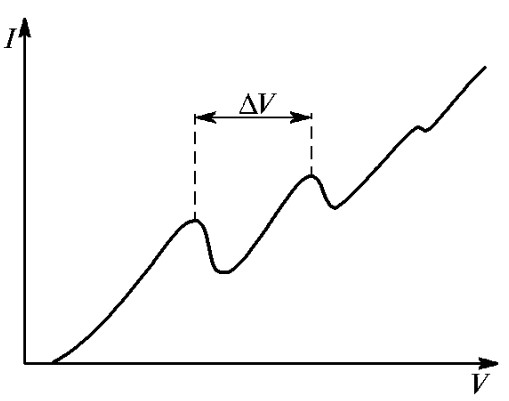
\includegraphics[scale=0.6]{../images/521-2}
\caption{Зависимость тока коллектора от напряжения на аноде}
\end{figure}

\section{Экспериментальная установка}

Для опыта используется серийная лампа ионизационного манометра ЛМ-2, заполненная гелием до давления ~1 Торр. Источником электронов является вольфрамолый катод, нагреваемый переменным током. Ток накала регулируется амперметром А. Ускоряющее напряжение подается на анод от выпрямителя В. Источник задерживающего напряжения -- батарея 4.5 В.

\begin{figure}[H]
\centering
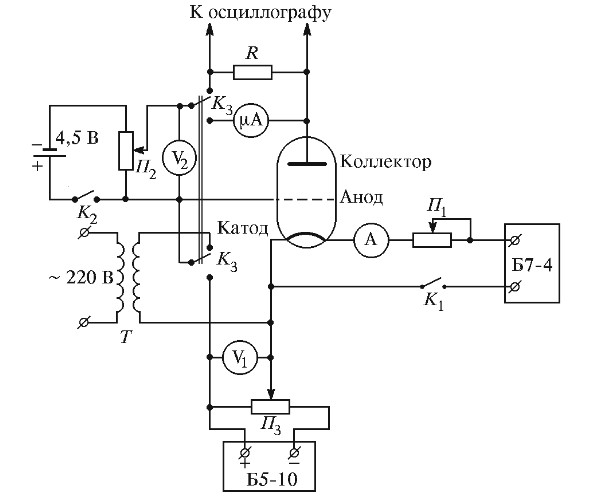
\includegraphics[scale=0.6]{../images/521-3}
\caption{Схема экспериментальной установки}
\end{figure}

Схему можно переключать из статического режима измерений в динамический  с помощью ключа $К_3$. При динамическом режиме ускоряющий потенциал подается с понижающего трансформатора Т.

\section{Проведение эксперимента}

\section{Обработка результатов}

\section{Выводы}

\end{document}